\section{Introduction}

\subsection{Matching}

    A \textbf{Matching} of \textit{graph}, $G$ is a \textit{subgraph} $M \subseteq G$ such that every edge shares no vertex with any other edge. That is, each vertex in matching $M$ has  degree \textbf{one}.
     
    The \textbf{size} of a matching is the number of edges in that matching.

\begin{figure}[ht]
    \begin{center}
  \includegraphics[width=0.4\textwidth]{IMAGES_FIGS/FIG_1_1.png}
  \caption{A Graph $G$ with $8$ vertices and $9$ edges.}
  \label{FIG_1_1}
  \end{center}
  
\end{figure}

In Figure \ref{FIG_1_1}, let's denote the edge that connects vertices $i$ and $j$ as $(i, j)$. Note that $\{(3, 8)\}$ is a \textit{matching}. The pairs $\{(3, 8),(4, 7)\}$ also make a \textit{matching} which is of size \textit{two}. Can we get a matching of size three? \textbf{Yes} !!!, it is $\{(2, 3),(4, 8),(5, 7)\}$. 


\subsection{Maximal matching}
    \begin{figure}[ht]
    \begin{center}
  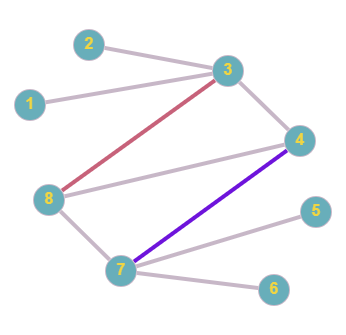
\includegraphics[width=0.4\textwidth]{IMAGES_FIGS/FIG_1_2.png}
  \caption{Coloured edges denoting the \textit{Maximal matching}}
  \label{FIG_1_2}
  \end{center}
  
\end{figure}

A \textbf{maximal matching} is a matching $M$ of the graph $G$, that is not a \textit{subset} of any other $matching$.
       
\textit{Example:} $\{(3, 8),(4, 7)\}$, It can't be a subset of any other Matching.
 

\subsection{Maximum matching}

A matching is \textbf{maximum} when it has the largest possible size. The \textbf{matching number} of a graph $G$ is the size of a \textit{maximum matching} of that graph.

    \begin{figure}[ht]
    \begin{center}
  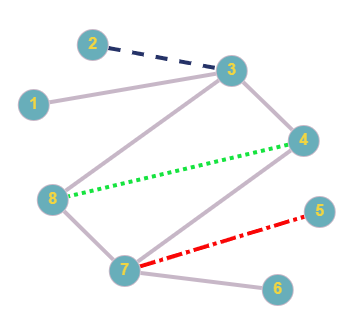
\includegraphics[width=0.4\textwidth]{IMAGES_FIGS/FIG_1_3.png}
  \caption{Coloured edges denoting the \textit{Maximum matching}}
  \label{FIG_1_3}
  \end{center}
  
\end{figure}


\textit{Note}: The \textbf{matching number} of the graph in Figure \ref{FIG_1_3} is $three$.
\newline
For a given graph $G$, there might be several \textit{maximum matchings}.
 

\subsection{Perfect Matching}

A matching $M$ of a graph $G$ is \textbf{perfect} if it contains all of the graph $G^\prime s$ vertices. 
That is, a matching is perfect if every vertex of the graph is incident to an edge of the matching. Every perfect matching is maximum and hence maximal.
\newline
\textit{Note} : \textbf{No perfect} matching exists for Figure \ref{FIG_1_4}.
\begin{figure}[ht]
\begin{center}
  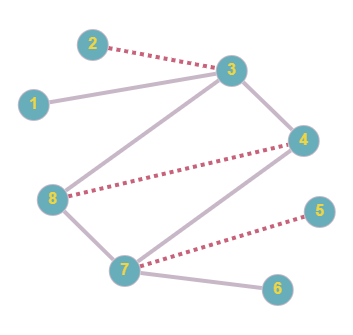
\includegraphics[width=0.4\textwidth]{IMAGES_FIGS/FIG_1_4.png}
  \caption{Dotted edges denoting the \textit{Perfect matching}}
  \label{FIG_1_4}
  \end{center}
  
\end{figure}

Well, a matching of size four means that every vertex is paired, but vertices $1$ and $2$ must both be paired with vertex $3$. So no, three is the best we can do. We call it a maximum matching.
 